\documentclass{standalone}
\usepackage{tikz}
\usetikzlibrary{patterns, positioning}


\begin{document}
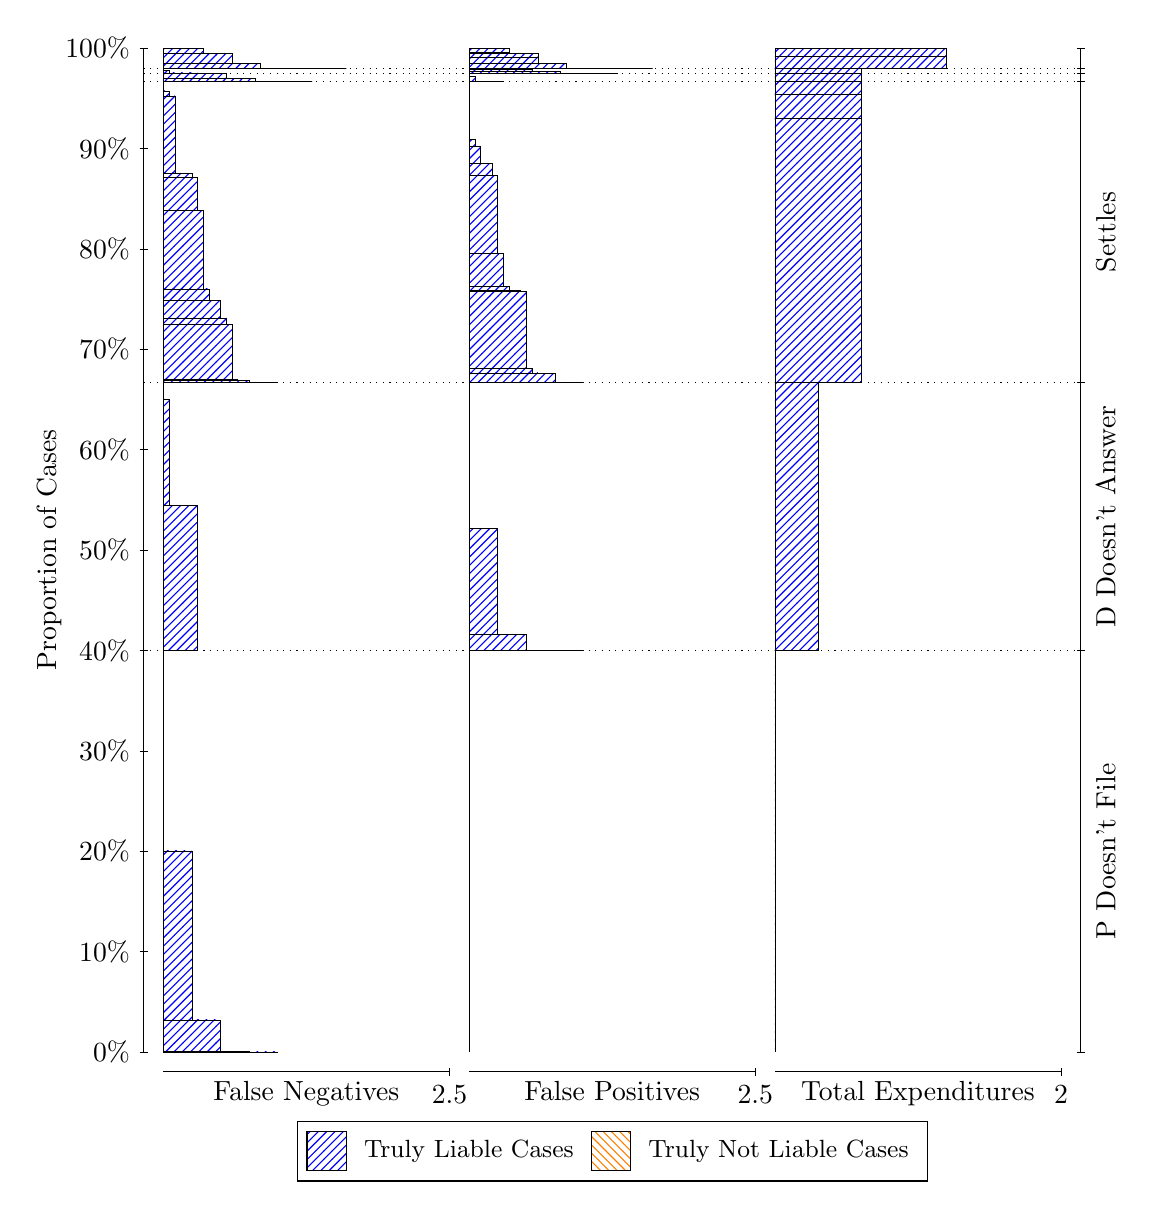
\begin{tikzpicture}
\draw[black, very thin] (1.5,1.75) -- (1.5,14.5);
\node[rotate=90, text=black, anchor=center] at (0.3, 8.125) {Proportion of Cases};
\draw[black, very thin] (1.45,1.75) -- (1.55,1.75);
\node[text=black, anchor=east] at (1.45, 1.75) {0\%};
\draw[black, very thin] (1.45,3.025) -- (1.55,3.025);
\node[text=black, anchor=east] at (1.45, 3.025) {10\%};
\draw[black, very thin] (1.45,4.3) -- (1.55,4.3);
\node[text=black, anchor=east] at (1.45, 4.3) {20\%};
\draw[black, very thin] (1.45,5.575) -- (1.55,5.575);
\node[text=black, anchor=east] at (1.45, 5.575) {30\%};
\draw[black, very thin] (1.45,6.85) -- (1.55,6.85);
\node[text=black, anchor=east] at (1.45, 6.85) {40\%};
\draw[black, very thin] (1.45,8.125) -- (1.55,8.125);
\node[text=black, anchor=east] at (1.45, 8.125) {50\%};
\draw[black, very thin] (1.45,9.4) -- (1.55,9.4);
\node[text=black, anchor=east] at (1.45, 9.4) {60\%};
\draw[black, very thin] (1.45,10.675) -- (1.55,10.675);
\node[text=black, anchor=east] at (1.45, 10.675) {70\%};
\draw[black, very thin] (1.45,11.95) -- (1.55,11.95);
\node[text=black, anchor=east] at (1.45, 11.95) {80\%};
\draw[black, very thin] (1.45,13.225) -- (1.55,13.225);
\node[text=black, anchor=east] at (1.45, 13.225) {90\%};
\draw[black, very thin] (1.45,14.5) -- (1.55,14.5);
\node[text=black, anchor=east] at (1.45, 14.5) {100\%};

\draw[black, very thin] (13.4,1.75) -- (13.4,14.5);
\draw[black, very thin] (13.35,1.75) -- (13.45,1.75);
\node[anchor=west] at (13.35, 1.75) {};
\draw[black, very thin] (13.35,6.8489) -- (13.45,6.8489);
\node[anchor=west] at (13.35, 6.8489) {};
\draw[black, very thin] (13.35,10.249) -- (13.45,10.249);
\node[anchor=west] at (13.35, 10.249) {};
\draw[black, very thin] (13.35,14.078) -- (13.45,14.078);
\node[anchor=west] at (13.35, 14.078) {};
\draw[black, very thin] (13.35,14.182) -- (13.45,14.182);
\node[anchor=west] at (13.35, 14.182) {};
\draw[black, very thin] (13.35,14.237) -- (13.45,14.237);
\node[anchor=west] at (13.35, 14.237) {};
\draw[black, very thin] (13.35,14.5) -- (13.45,14.5);
\node[anchor=west] at (13.35, 14.5) {};

\draw[black, very thin, pattern color=blue, pattern=north east lines] (1.75,1.75) rectangle (3.2033,1.75);
\draw[black, very thin, pattern color=blue, pattern=north east lines] (1.75,1.75) rectangle (2.84,1.7534);
\draw[black, very thin, pattern color=blue, pattern=north east lines] (1.75,1.7534) rectangle (2.4767,2.158);
\draw[black, very thin, pattern color=blue, pattern=north east lines] (1.75,2.158) rectangle (2.1133,4.3029);
\draw[black, very thin, pattern color=orange, pattern=north west lines] (1.75,4.3029) rectangle (1.75,4.3029);
\draw[black, very thin, pattern color=blue, pattern=north east lines] (1.75,4.3029) rectangle (1.75,6.8489);
\draw[black, very thin, pattern color=blue, pattern=north east lines] (1.75,6.8489) rectangle (2.186,8.6953);
\draw[black, very thin, pattern color=blue, pattern=north east lines] (1.75,8.6953) rectangle (1.8227,10.044);
\draw[black, very thin, pattern color=orange, pattern=north west lines] (1.75,10.044) rectangle (1.75,10.044);
\draw[black, very thin, pattern color=blue, pattern=north east lines] (1.75,10.044) rectangle (1.75,10.249);
\draw[black, very thin, pattern color=blue, pattern=north east lines] (1.75,10.249) rectangle (3.2033,10.249);
\draw[black, very thin, pattern color=blue, pattern=north east lines] (1.75,10.249) rectangle (3.058,10.249);
\draw[black, very thin, pattern color=blue, pattern=north east lines] (1.75,10.249) rectangle (2.9127,10.249);
\draw[black, very thin, pattern color=blue, pattern=north east lines] (1.75,10.249) rectangle (2.84,10.28);
\draw[black, very thin, pattern color=blue, pattern=north east lines] (1.75,10.28) rectangle (2.6947,10.288);
\draw[black, very thin, pattern color=blue, pattern=north east lines] (1.75,10.288) rectangle (2.622,10.989);
\draw[black, very thin, pattern color=blue, pattern=north east lines] (1.75,10.989) rectangle (2.5493,11.073);
\draw[black, very thin, pattern color=blue, pattern=north east lines] (1.75,11.073) rectangle (2.4767,11.293);
\draw[black, very thin, pattern color=blue, pattern=north east lines] (1.75,11.293) rectangle (2.3313,11.441);
\draw[black, very thin, pattern color=blue, pattern=north east lines] (1.75,11.441) rectangle (2.2587,12.437);
\draw[black, very thin, pattern color=blue, pattern=north east lines] (1.75,12.437) rectangle (2.186,12.853);
\draw[black, very thin, pattern color=blue, pattern=north east lines] (1.75,12.853) rectangle (2.1133,12.906);
\draw[black, very thin, pattern color=blue, pattern=north east lines] (1.75,12.906) rectangle (1.968,12.914);
\draw[black, very thin, pattern color=blue, pattern=north east lines] (1.75,12.914) rectangle (1.8953,13.893);
\draw[black, very thin, pattern color=blue, pattern=north east lines] (1.75,13.893) rectangle (1.8227,13.955);
\draw[black, very thin, pattern color=orange, pattern=north west lines] (1.75,13.955) rectangle (1.75,13.955);
\draw[black, very thin, pattern color=blue, pattern=north east lines] (1.75,13.955) rectangle (1.75,14.078);
\draw[black, very thin, pattern color=blue, pattern=north east lines] (1.75,14.078) rectangle (3.6393,14.078);
\draw[black, very thin, pattern color=blue, pattern=north east lines] (1.75,14.078) rectangle (3.276,14.078);
\draw[black, very thin, pattern color=blue, pattern=north east lines] (1.75,14.078) rectangle (2.9127,14.117);
\draw[black, very thin, pattern color=blue, pattern=north east lines] (1.75,14.117) rectangle (2.5493,14.181);
\draw[black, very thin, pattern color=blue, pattern=north east lines] (1.75,14.181) rectangle (2.186,14.182);
\draw[black, very thin, pattern color=orange, pattern=north west lines] (1.75,14.182) rectangle (1.75,14.182);
\draw[black, very thin, pattern color=blue, pattern=north east lines] (1.75,14.182) rectangle (2.186,14.183);
\draw[black, very thin, pattern color=blue, pattern=north east lines] (1.75,14.183) rectangle (1.8227,14.216);
\draw[black, very thin, pattern color=orange, pattern=north west lines] (1.75,14.216) rectangle (1.75,14.216);
\draw[black, very thin, pattern color=blue, pattern=north east lines] (1.75,14.216) rectangle (1.75,14.237);
\draw[black, very thin, pattern color=blue, pattern=north east lines] (1.75,14.237) rectangle (4.0753,14.237);
\draw[black, very thin, pattern color=blue, pattern=north east lines] (1.75,14.237) rectangle (3.712,14.237);
\draw[black, very thin, pattern color=blue, pattern=north east lines] (1.75,14.237) rectangle (3.3487,14.241);
\draw[black, very thin, pattern color=blue, pattern=north east lines] (1.75,14.241) rectangle (2.9853,14.301);
\draw[black, very thin, pattern color=blue, pattern=north east lines] (1.75,14.301) rectangle (2.622,14.434);
\draw[black, very thin, pattern color=blue, pattern=north east lines] (1.75,14.434) rectangle (2.2587,14.495);
\draw[black, very thin, pattern color=blue, pattern=north east lines] (1.75,14.495) rectangle (1.8953,14.5);
\draw[black, very thin, pattern color=orange, pattern=north west lines] (1.75,14.5) rectangle (1.75,14.5);
\draw[black, very thin, pattern color=blue, pattern=north east lines] (1.75,14.5) rectangle (1.75,14.5);
\draw[black, very thin, pattern color=orange, pattern=north west lines] (5.6333,1.75) rectangle (5.6333,1.75);
\draw[black, very thin, pattern color=blue, pattern=north east lines] (5.6333,1.75) rectangle (5.6333,6.8489);
\draw[black, very thin, pattern color=orange, pattern=north west lines] (5.6333,6.8489) rectangle (7.0867,6.8489);
\draw[black, very thin, pattern color=blue, pattern=north east lines] (5.6333,6.8489) rectangle (7.0867,6.8489);
\draw[black, very thin, pattern color=blue, pattern=north east lines] (5.6333,6.8489) rectangle (6.7233,6.8492);
\draw[black, very thin, pattern color=blue, pattern=north east lines] (5.6333,6.8492) rectangle (6.36,7.0541);
\draw[black, very thin, pattern color=blue, pattern=north east lines] (5.6333,7.0541) rectangle (5.9967,8.4024);
\draw[black, very thin, pattern color=blue, pattern=north east lines] (5.6333,8.4024) rectangle (5.6333,10.249);
\draw[black, very thin, pattern color=orange, pattern=north west lines] (5.6333,10.249) rectangle (7.0867,10.249);
\draw[black, very thin, pattern color=blue, pattern=north east lines] (5.6333,10.249) rectangle (7.0867,10.249);
\draw[black, very thin, pattern color=orange, pattern=north west lines] (5.6333,10.249) rectangle (6.796,10.249);
\draw[black, very thin, pattern color=blue, pattern=north east lines] (5.6333,10.249) rectangle (6.796,10.249);
\draw[black, very thin, pattern color=blue, pattern=north east lines] (5.6333,10.249) rectangle (6.7233,10.372);
\draw[black, very thin, pattern color=orange, pattern=north west lines] (5.6333,10.372) rectangle (6.6507,10.372);
\draw[black, very thin, pattern color=blue, pattern=north east lines] (5.6333,10.372) rectangle (6.6507,10.372);
\draw[black, very thin, pattern color=orange, pattern=north west lines] (5.6333,10.372) rectangle (6.5053,10.372);
\draw[black, very thin, pattern color=blue, pattern=north east lines] (5.6333,10.372) rectangle (6.5053,10.373);
\draw[black, very thin, pattern color=blue, pattern=north east lines] (5.6333,10.373) rectangle (6.4327,10.434);
\draw[black, very thin, pattern color=blue, pattern=north east lines] (5.6333,10.434) rectangle (6.36,11.413);
\draw[black, very thin, pattern color=blue, pattern=north east lines] (5.6333,11.413) rectangle (6.2873,11.421);
\draw[black, very thin, pattern color=blue, pattern=north east lines] (5.6333,11.421) rectangle (6.142,11.474);
\draw[black, very thin, pattern color=blue, pattern=north east lines] (5.6333,11.474) rectangle (6.0693,11.891);
\draw[black, very thin, pattern color=blue, pattern=north east lines] (5.6333,11.891) rectangle (5.9967,12.886);
\draw[black, very thin, pattern color=blue, pattern=north east lines] (5.6333,12.886) rectangle (5.924,13.035);
\draw[black, very thin, pattern color=blue, pattern=north east lines] (5.6333,13.035) rectangle (5.7787,13.254);
\draw[black, very thin, pattern color=blue, pattern=north east lines] (5.6333,13.254) rectangle (5.706,13.338);
\draw[black, very thin, pattern color=blue, pattern=north east lines] (5.6333,13.338) rectangle (5.6333,14.078);
\draw[black, very thin, pattern color=orange, pattern=north west lines] (5.6333,14.078) rectangle (6.0693,14.078);
\draw[black, very thin, pattern color=blue, pattern=north east lines] (5.6333,14.078) rectangle (6.0693,14.08);
\draw[black, very thin, pattern color=blue, pattern=north east lines] (5.6333,14.08) rectangle (5.706,14.143);
\draw[black, very thin, pattern color=blue, pattern=north east lines] (5.6333,14.143) rectangle (5.6333,14.182);
\draw[black, very thin, pattern color=orange, pattern=north west lines] (5.6333,14.182) rectangle (7.5227,14.182);
\draw[black, very thin, pattern color=blue, pattern=north east lines] (5.6333,14.182) rectangle (7.5227,14.182);
\draw[black, very thin, pattern color=blue, pattern=north east lines] (5.6333,14.182) rectangle (7.1593,14.182);
\draw[black, very thin, pattern color=blue, pattern=north east lines] (5.6333,14.182) rectangle (6.796,14.203);
\draw[black, very thin, pattern color=blue, pattern=north east lines] (5.6333,14.203) rectangle (6.4327,14.236);
\draw[black, very thin, pattern color=blue, pattern=north east lines] (5.6333,14.236) rectangle (6.0693,14.237);
\draw[black, very thin, pattern color=orange, pattern=north west lines] (5.6333,14.237) rectangle (7.9587,14.237);
\draw[black, very thin, pattern color=blue, pattern=north east lines] (5.6333,14.237) rectangle (7.9587,14.237);
\draw[black, very thin, pattern color=orange, pattern=north west lines] (5.6333,14.237) rectangle (7.5953,14.237);
\draw[black, very thin, pattern color=blue, pattern=north east lines] (5.6333,14.237) rectangle (7.5953,14.237);
\draw[black, very thin, pattern color=orange, pattern=north west lines] (5.6333,14.237) rectangle (7.232,14.237);
\draw[black, very thin, pattern color=blue, pattern=north east lines] (5.6333,14.237) rectangle (7.232,14.242);
\draw[black, very thin, pattern color=blue, pattern=north east lines] (5.6333,14.242) rectangle (6.8687,14.302);
\draw[black, very thin, pattern color=orange, pattern=north west lines] (5.6333,14.302) rectangle (6.8687,14.302);
\draw[black, very thin, pattern color=blue, pattern=north east lines] (5.6333,14.302) rectangle (6.8687,14.303);
\draw[black, very thin, pattern color=blue, pattern=north east lines] (5.6333,14.303) rectangle (6.5053,14.386);
\draw[black, very thin, pattern color=orange, pattern=north west lines] (5.6333,14.386) rectangle (6.5053,14.386);
\draw[black, very thin, pattern color=blue, pattern=north east lines] (5.6333,14.386) rectangle (6.5053,14.435);
\draw[black, very thin, pattern color=blue, pattern=north east lines] (5.6333,14.435) rectangle (6.142,14.447);
\draw[black, very thin, pattern color=blue, pattern=north east lines] (5.6333,14.447) rectangle (6.142,14.496);
\draw[black, very thin, pattern color=blue, pattern=north east lines] (5.6333,14.496) rectangle (5.7787,14.496);
\draw[black, very thin, pattern color=blue, pattern=north east lines] (5.6333,14.496) rectangle (5.7787,14.5);
\draw[black, very thin, pattern color=blue, pattern=north east lines] (5.6333,14.5) rectangle (5.6333,14.5);
\draw[black, very thin, pattern color=orange, pattern=north west lines] (9.5167,1.75) rectangle (9.5167,1.75);
\draw[black, very thin, pattern color=blue, pattern=north east lines] (9.5167,1.75) rectangle (9.5167,6.8489);
\draw[black, very thin, pattern color=orange, pattern=north west lines] (9.5167,6.8489) rectangle (10.062,6.8489);
\draw[black, very thin, pattern color=blue, pattern=north east lines] (9.5167,6.8489) rectangle (10.062,10.249);
\draw[black, very thin, pattern color=orange, pattern=north west lines] (9.5167,10.249) rectangle (10.607,10.249);
\draw[black, very thin, pattern color=blue, pattern=north east lines] (9.5167,10.249) rectangle (10.607,13.61);
\draw[black, very thin, pattern color=orange, pattern=north west lines] (9.5167,13.61) rectangle (10.607,13.61);
\draw[black, very thin, pattern color=blue, pattern=north east lines] (9.5167,13.61) rectangle (10.607,13.914);
\draw[black, very thin, pattern color=orange, pattern=north west lines] (9.5167,13.914) rectangle (10.607,13.914);
\draw[black, very thin, pattern color=blue, pattern=north east lines] (9.5167,13.914) rectangle (10.607,14.078);
\draw[black, very thin, pattern color=orange, pattern=north west lines] (9.5167,14.078) rectangle (10.607,14.078);
\draw[black, very thin, pattern color=blue, pattern=north east lines] (9.5167,14.078) rectangle (10.607,14.182);
\draw[black, very thin, pattern color=orange, pattern=north west lines] (9.5167,14.182) rectangle (10.607,14.182);
\draw[black, very thin, pattern color=blue, pattern=north east lines] (9.5167,14.182) rectangle (10.607,14.237);
\draw[black, very thin, pattern color=orange, pattern=north west lines] (9.5167,14.237) rectangle (11.697,14.237);
\draw[black, very thin, pattern color=blue, pattern=north east lines] (9.5167,14.237) rectangle (11.697,14.396);
\draw[black, very thin, pattern color=orange, pattern=north west lines] (9.5167,14.396) rectangle (11.697,14.396);
\draw[black, very thin, pattern color=blue, pattern=north east lines] (9.5167,14.396) rectangle (11.697,14.5);
\draw[black, dotted] (1.5,6.8489) -- (13.4,6.8489);
\draw[black, dotted] (1.5,10.249) -- (13.4,10.249);
\draw[black, dotted] (1.5,14.078) -- (13.4,14.078);
\draw[black, dotted] (1.5,14.182) -- (13.4,14.182);
\draw[black, dotted] (1.5,14.237) -- (13.4,14.237);
\draw[black, very thin] (1.75,1.5) -- (5.3833,1.5);
\node[text=black, anchor=north] at (3.5667, 1.5) {False Negatives};
\draw[black, very thin] (5.3833,1.45) -- (5.3833,1.55);
\node[text=black, anchor=north] at (5.3833, 1.45) {2.5};

\draw[black, very thin] (5.6333,1.5) -- (9.2667,1.5);
\node[text=black, anchor=north] at (7.45, 1.5) {False Positives};
\draw[black, very thin] (9.2667,1.45) -- (9.2667,1.55);
\node[text=black, anchor=north] at (9.2667, 1.45) {2.5};

\draw[black, very thin] (9.5167,1.5) -- (13.15,1.5);
\node[text=black, anchor=north] at (11.333, 1.5) {Total Expenditures};
\draw[black, very thin] (13.15,1.45) -- (13.15,1.55);
\node[text=black, anchor=north] at (13.15, 1.45) {2};

\node[text=black, centered, rotate=90] at (13.72, 4.2994) {P Doesn't File};
\node[text=black, centered, rotate=90] at (13.72, 8.5489) {D Doesn't Answer};
\node[text=black, centered, rotate=90] at (13.72, 12.164) {Settles};




\draw (7.449999999999999,1.5) node[draw=none] (baseCoordinate) {};
\begin{scope}[align=center]
        \matrix[scale=0.5, draw=black, below=0.5cm of baseCoordinate, nodes={draw}, column sep=0.1cm]{
            \node[rectangle, draw, minimum width=0.5cm, minimum height=0.5cm, pattern color=blue, pattern=north east lines] {}; &
            \node[draw=none, font=\small, text=black] (B) {Truly Liable Cases}; &
            \node[rectangle, draw, minimum width=0.5cm, minimum height=0.5cm, pattern color=orange, pattern=north west lines] {}; &
            \node[draw=none, font=\small, text=black] (B) {Truly Not Liable Cases}; \\
            };
\end{scope}

\end{tikzpicture}
\end{document}